\section{Intelligence Artificielle}

\subsection{Stratégies}

\subsubsection{Intelligence aléatoire}
Cette stratégie consiste en un joueur qui a chaque étape du jeu aurait le choix entre plusieurs options et en choisit une de manière aléatoire.

\newpage
\subsection{Conception logiciel}
Le diagramme des classes pour l’intelligence artificielle est présenté en figure \ref{fig:ai}.

\textbf{Les CLasses AI} : Les classes héritières de AI implémente plusieurs stratégies d'intelligence artificielle.
\begin{itemize}
    \item RamdomAI : Intelligence aléatoire
\end{itemize}

\begin{landscape}
    \begin{figure}[!htbp]
        \centering
        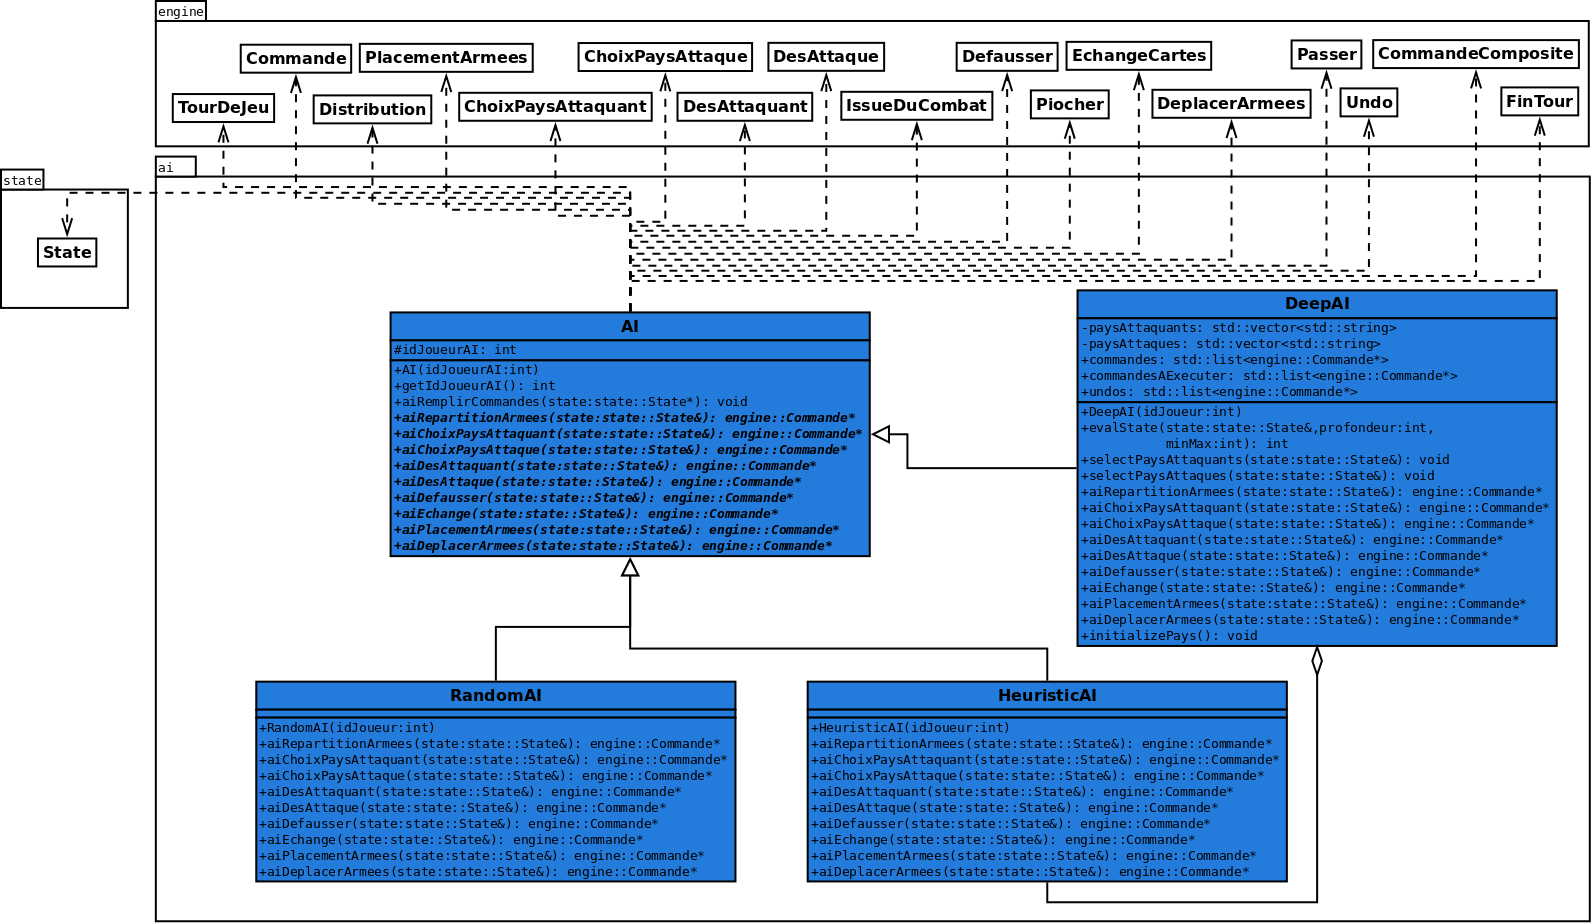
\includegraphics[width=17cm]{Images/ai.png}
        \caption{Diagramme de l'intelligence artificielle}
        \label{fig:ai}
    \end{figure}
\end{landscape}